%data
\section{Point Source Tracks Sample}
which dataset to use and why\\
description of the set: table of various info (livetime, number of events)\\
mention overlap in time due to testruns\\

\section{Monte Carlo Pre-Processing}
removing sources from data and mc\\
show sindec distribution of mc and filtered mc, maybe sindec-energy 2d hist\\
mention weighting (Powerlawflux)\\

Since GFU-gold events are treated as sources, keeping these events in the dataset would lead to a bias, due to essentially double counting them as events and sources.
Alert events in general are excluded from the Point Source Tracks Sample starting with IC86.
Some alerts do appear in IC76 and previous runs because these datasets are too old, but are excluded in this analysis since it starts with the year 2011.
Following a conservative approach, GFU-gold like events also have to be identified and removed from the simulation files.
Luckily all datasets from the years 2011 to 2019 use the monte carlo file from the year 2016, so this is the only simulation set that needs to be worked with.\\
To identify the GFU-gold events from the monte carlo set, the original i3 simulation files and the corresponding geometry file (GCD: geometry, something c, detector configuration) file need to be found and processed using the alertfilter from realtime.
The matching simulation files are 21002 and 21220.
Information about these sets can be found at \cite{sim} and \cite{gcd} for the geometry file.
It is important to mention that the events in the final monte carlo set cannot be identified by their ids, since these values were replaced by the job-id of the corresponding iceprod job which processed these to the final level. An exeption is the run-id.
The temporal parameter can also not be used, since all event times in the final monte carlo are set to \num{0}.
The event times will be generated later in the analysis to match the analysis framework.
The identification has to be done via other parameters like zenith and azimuth.
Additionally the true energy was also taken as an identifying parameter to rule out any events coincidentially appearing from the same direction.
A comparison of the sindec distribution of the real GFU-gold alerts and the GFU-gold simulation events can be seen in figure \ref{fig:gfu-gold-comp}.

\begin{figure}
    \centering
    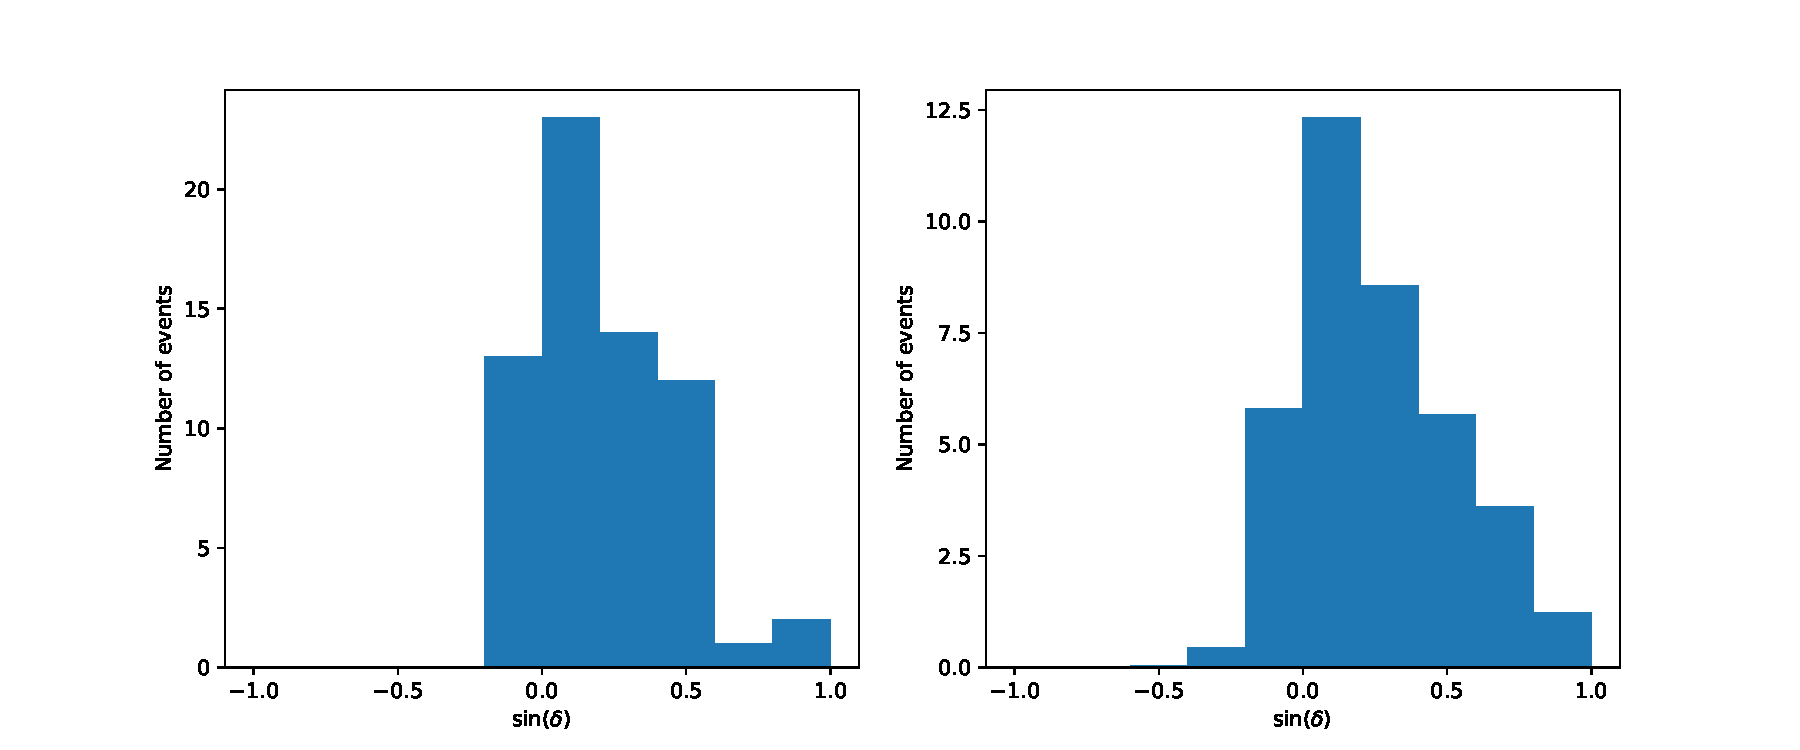
\includegraphics[width=\linewidth]{Plots/03_data/gfu_gold_comp.pdf}
    \label{fig:gfu-gold-comp}
    \caption{The sine declination of the real GFU-gold alerts over 9 years used in this analysis (left) and the GFU-gold simulation events from the mc 2016 sample (right). The simulation events have been weighted with a livetime of 9 years and flux from \cite{flux}.}
\end{figure}

The filtered events can also be seen in figure \ref{fig:energy}.

\begin{figure}
    \centering
    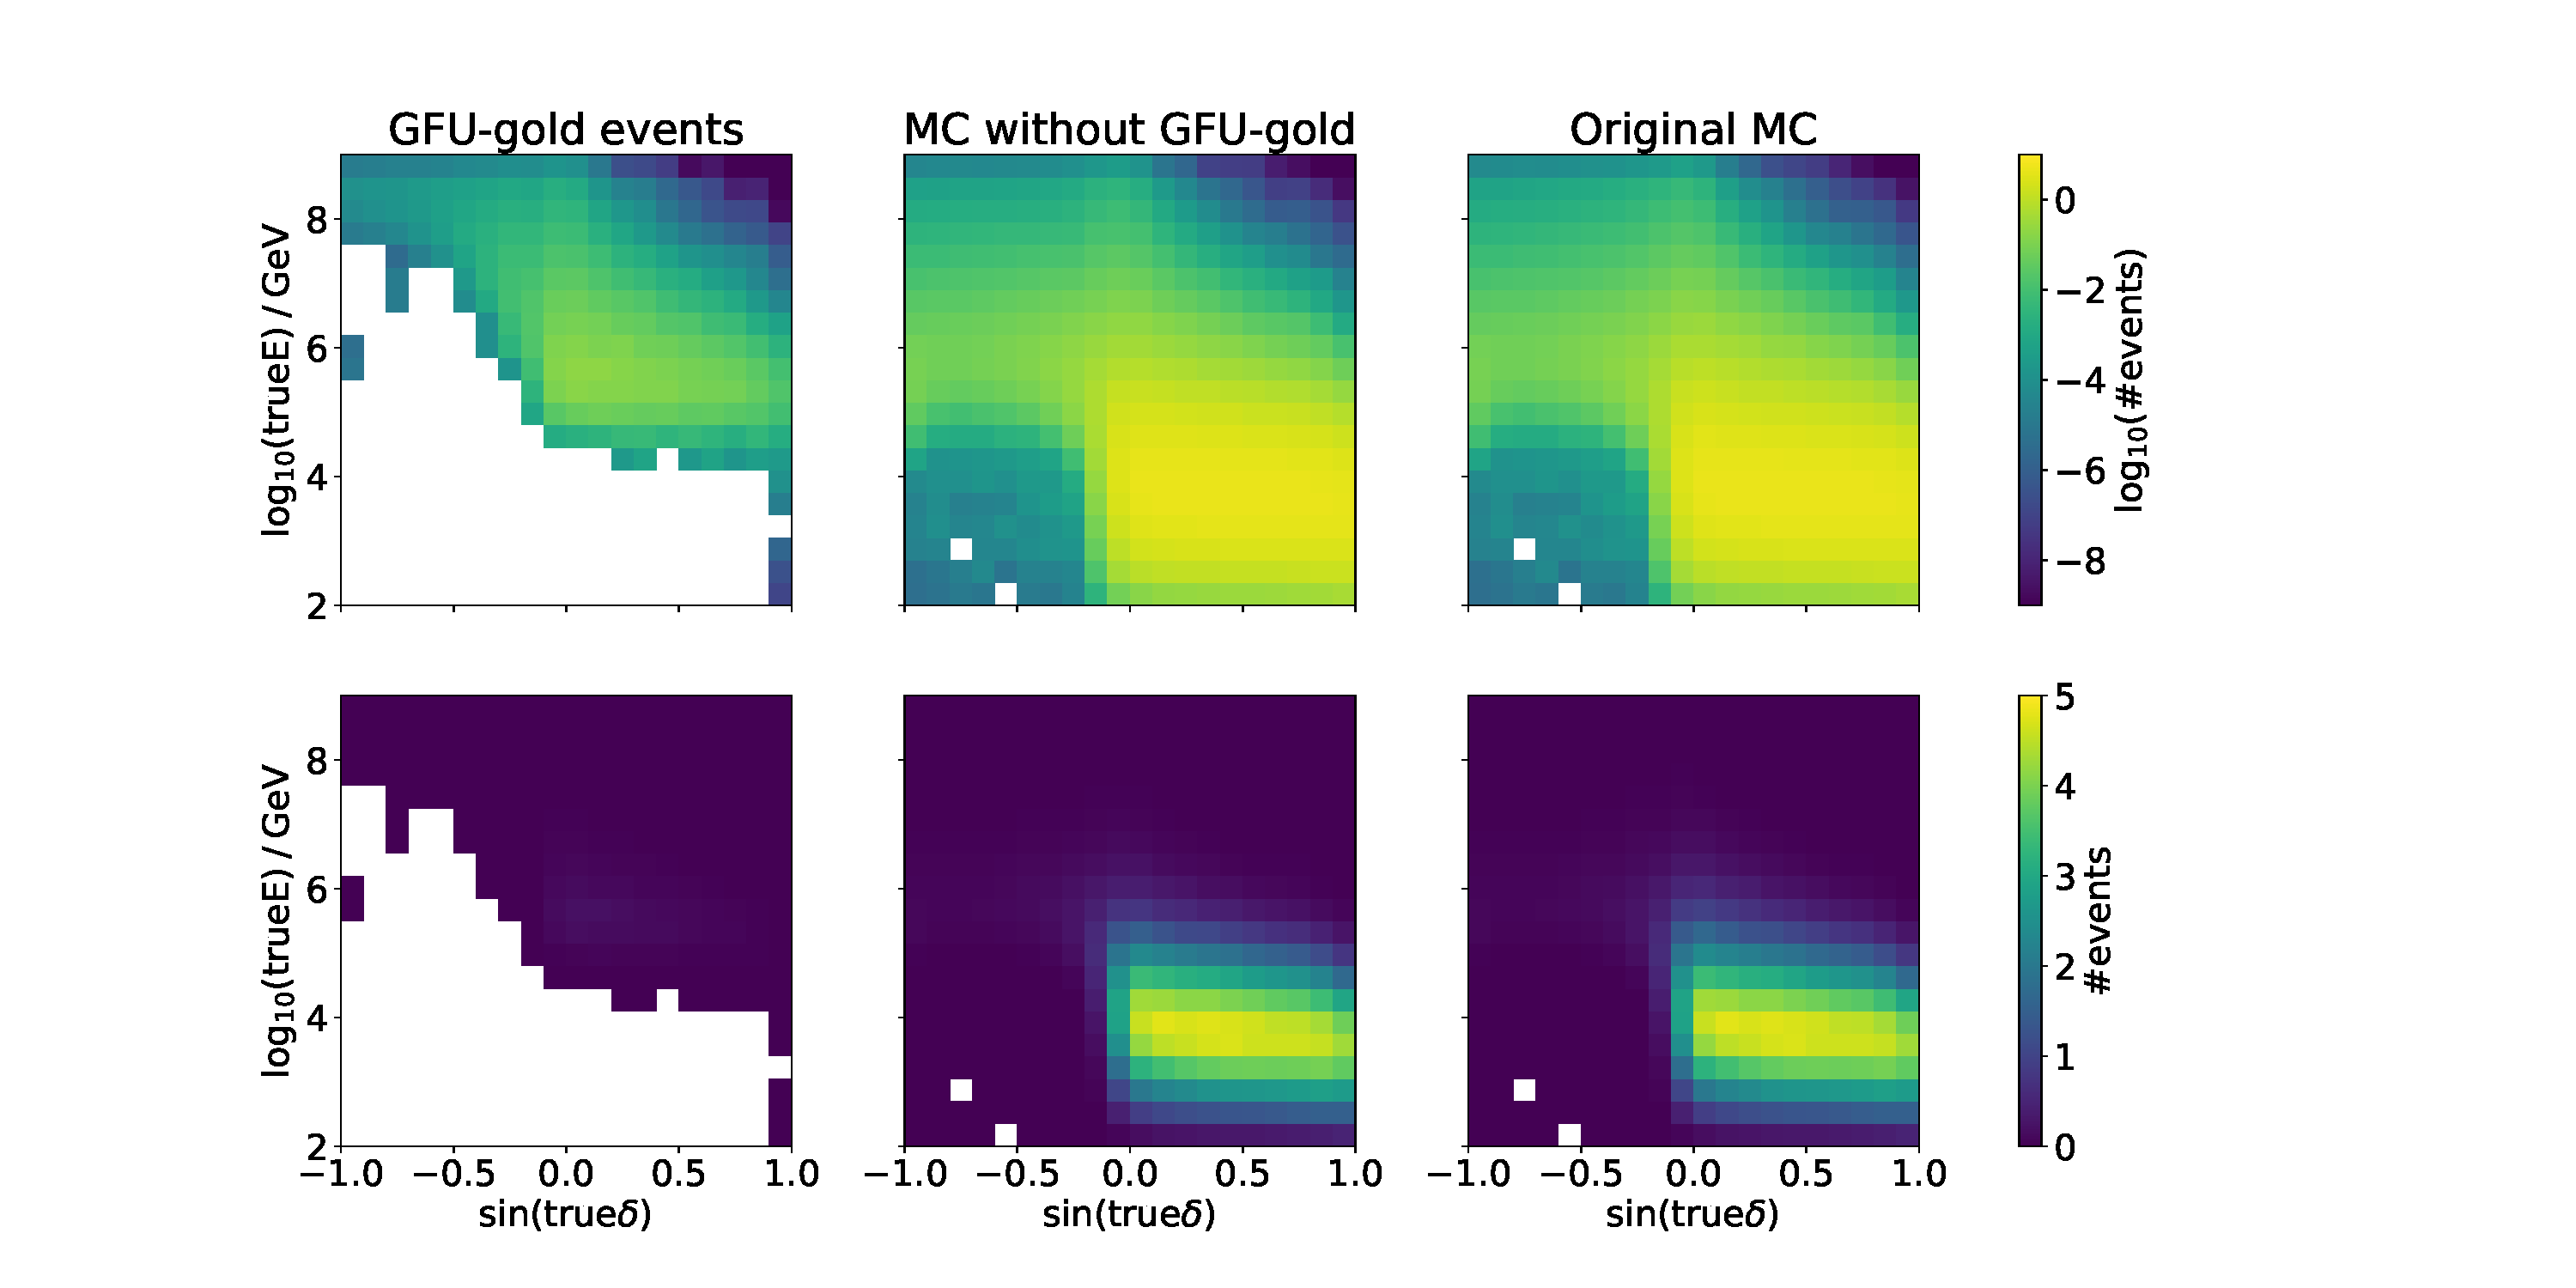
\includegraphics[width=\linewidth]{Plots/03_data/cleaned_mc_energy_test.pdf}
    \label{fig:energy}
    \caption{.}
\end{figure}
